\subsection{Single Responsibility Principle} \label{srp}

\evaluatePrincipleTable{\acrshort{srp}}{table_srp_convergence}{ \addEvalRow{\gls{soc} &
    \fullConvergence & The main goal of both \gls{srp} and \gls{soc} is to promote and
    encourage modularity, low coupling, and high cohesion. While the definition has some
    differences, the two principles are practically interchangeable. Many examples in the
    Artifacts show a strong convergence between \gls{srp} and \gls{soc}. To name one, an
    Expander should be able to can perform multiple Tasks to complete the full
    instantiation of the model. Each of those Tasks can be implemented separately from
    each other. Figure \ref{fig_handlers} illustrates some of the Tasks implemented in the
    Clean Architecture Expander artifact. The Code Listing
    \ref{list_expandentitieshandlerinteractor} is an example of one implementation of such
    a task \citecode{koks_expandentitieshandlerinteractor_2023}.}
    
    \addEvalRow{\gls{dvt} & \npartialConvergence & Although using SRP does not implicitly
    guarantee \gls{dvt}, it supports \gls{dvt} by directing certain design choices.For
    example, \gls{ca} and \gls{ns} assign specific \gls{dto} objects to support specific
    use cases (Interactors or Tasks) or transfer (parts of) Data between architectural
    layers. \gls{ca} specifically assigned \glspl{dto} and guidelines on where and when to
    use them. These are also applied in the artifact of this study as ResponseModels,
    RequestModels, and ViewModels
    \parencites{koks_requestmodels_2023,koks_viewmodels_2023}. The separation of data
    structures specific to Use Cases minimizes the impact of data structure changes by
    preferring stamp coupling over data coupling. However, \gls{srp} is not a guaranteed
    measure for \gls{dvt}.}
    
    \addEvalRow{\gls{avt} & \npartialConvergence & While \gls{srp} emphasizes limiting the
    responsibility of each module, it does not explicitly require handling specific
    versions of use cases. Nevertheless, adhering to \gls{srp} can still indirectly
    contribute to achieving \gls{avt}. One way to achieve this is by separating versions
    of Actions into separate contracts, objects, or methods, enabling Action Version
    transparency to some degree. Although not yet available in the artifact, Code Listing
    \ref{list_versioning} shows that API versioning is a common standard practice fully
    supported by the open API specification and the .net core framework
    \parencites{github_aspnet-api-versioningprogramcs_2023, oas_versioning_2023}.
    Manifestations in the artifact can be located in the Logger (Code Listing
    \ref{list_logging}), amongst others \parencite{koks_logger_2023}.}
    
    \addEvalRow{\gls{sos} &\noConvergence & Following \gls{srp} might lead to separate modules
    that manage their state, indirectly contributing to \gls{sos}. However, the convergence
    is very weak, and no manifestations are found in the artifacts.}

}

\begin{figure}[H]
    \centering
    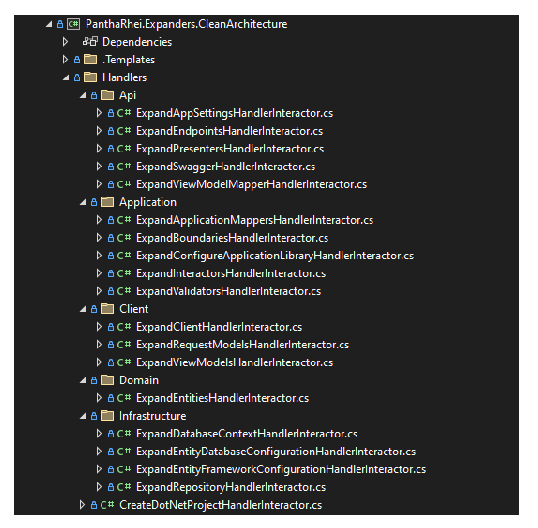
\includegraphics[width=0.6\textwidth]{figures/expander_handlers.pdf}
    \caption[The Clean Architecture Expander handlers]{Each of the handlers handles an isolated part of the expanding process.}
    \label{fig_handlers}
\end{figure}